%%%%%%齋藤研究室レジュメテンプレート%%%%%%% 2024

\documentclass[a4j]{jsarticle}
\usepackage[utf8]{inputenc}
\usepackage{amsmath,amssymb,amscd,amsthm}
\usepackage{ascmac,fancybox} 
\usepackage{bm}
\usepackage{mathtools}
\usepackage{multicol}
\usepackage{graphicx}
\usepackage[dvipdfmx]{color}
\usepackage{algorithm}%擬似コードを書く場合
\usepackage{algorithmic}%擬似コードを書く場合
\usepackage{url}
\usepackage[en-US]{datetime2}
\usepackage{diagbox}
%%%% ↓algotithmic の \REQUIRE と \ENSURE の表記を変更する
\renewcommand{\algorithmicrequire}{\textbf{Input:}}
\renewcommand{\algorithmicensure}{\textbf{Output:}}
%%%% ↑algotithmic の \REQUIRE と \ENSURE の表記を変更する
\def \QED{\hfill $\Box$}%証明終了の記号


%%%%%%%本文%%%%%%% 
\title{第1回\\学部3年後期ゼミナール発表資料}
\author{青山和樹}
\date{2024年10月7日}




\begin{document}

\maketitle

%%目的%%
\section*{発表の目的}
テキスト\cite{text}の
\begin{itemize}
	\item 2.1 Entropy
	\item 2.2 Joint entropy and conditional entropy
\end{itemize}
について発表する.


%%目次%%
\tableofcontents

\clearpage

%%本文%%

\section{Entropy}

まず確率変数の不確実性の尺度としてエントロピー(entropy)を導入する. Xをアルファベット$\mathcal{X}$の離散確率変数(discrete random variable)とし, その確率質量関数(probability mass function)を$p(x) = Pr(X = x), x \in \mathcal{X}$とする.\\

\textgt{注意 1.1} 確率質量関数を$px(x)$ではなく簡便のため$p(x)$と表しす. したがって, $p(x)$と$p(y)$は異なる確率変数に対して異なる確率質量関数$px(x)$と$py(y)$を指す. また以降, 確率関数を書く. \\

\begin{itembox}[l]{\textgt{定義 1.2} (エントロピー)}
	\begin{align}
		H(X) = - \sum_{x \in \mathcal{X}} p(x) \log p(x)
	\end{align}
	また, この量を$H(p)$とも書く. 対数は2を底とし, エントロピーはビット(bit)で表される.
\end{itembox}\\


\textgt{注意 1.3} $0 \log 0 = 0$ という規約を用いる, これは$x \log x$が$x \rightarrow 0$で0に収束するため, 連続性から容易に正当化される. よってゼロ確率の項を加えてもエントロピーは変わらない.\\

もし対数の底が$b$であれば, エントロピーは$H_b(X)$と表される. 対数の底が$e$の場合, エントロピーはナット(nat)で測定される. 特に指定がない限り, すべての対数は底2であり, したがってエントロピーはビットで測定されると考える. エントロピーは$X$の分布の汎関数であり, 実際に確率変数$X$が取る値には依存せず, 確率だけに依存する.\\

期待値は$E$によって表される. もし$X$が$p(x)$に従うならば, 確率変数$g(X)$の期待値は以下によって表される.

\begin{align}
	E_{p}g(X) = \sum_{x \in \mathcal{X}} g(x) p(x)
\end{align}

あるいは, 文脈から確率関数が明らかであれば, 単に$Eg(X)$と書く.\\

\textgt{解説 1.4} $X$のエントロピーは, 確率関数$p(x)$に従って$X$を選んだ場合の確率変数$\log \frac{1}{p(x)}$の期待値としても解釈できる. したがって,
\begin{align}
	H(X) = E_{p} \log \frac{1}{p(X)}
\end{align}
と表される.\\

\begin{itembox}[l]{\textgt{補題 1.5}}
	\begin{equation}
		H(X) \geq 0
	\end{equation}
\end{itembox}\\

\textgt{証明 1.6} $0 \leq p(x) \leq 1$であるから, $\log \frac{1}{p(x)} \geq 0$である. \qed\\

\begin{itembox}[l]{\textgt{補題 1.7}}
	\begin{equation}
		H_b(X) = (\log_b a)H_a(X)
	\end{equation}
\end{itembox}\\

\textgt{証明 1.8} $\log_b q = \log_b a \log_a p$. \qed\\

エントロピーの第2の性質として, 定義における対数の底を変更できることがある. エントロピーは, 適切な係数を掛けることで, 異なる底に変換できる.\\

\textgt{例 1.9}

\begin{align}
	X = \begin{cases}
		 & 1\:\:\:\mbox{確率}p\mbox{のとき},   \\
		 & 0\:\:\:\mbox{確率}1-p\mbox{のとき}.
	\end{cases}
\end{align}
のとき
\begin{align}
	H(X) = -p \log p - (1-p) \log (1-p) \stackrel{\mathrm{def}}{=} H(p)
\end{align}
特に$p = \frac{1}{2}$のとき$H(X) = 1$である. 関数$H(p)$のグラフは図\ref{fig:entropy}に示した. この図はエントロピーの基本的な性質を示しており, エントロピーは分布に対して凹関数であり, $p = 0$または$1$のとき$0$となる. これは, $p = 0$または$1$の場合, 変数はランダムでなくなり, 不確実性がなくなるためである. 同様に, 不確実性が最大となるのは$p = \frac{1}{2}$のときであり, このときエントロピーも最大値を取る.\\

\begin{figure}[H]
	\centering
	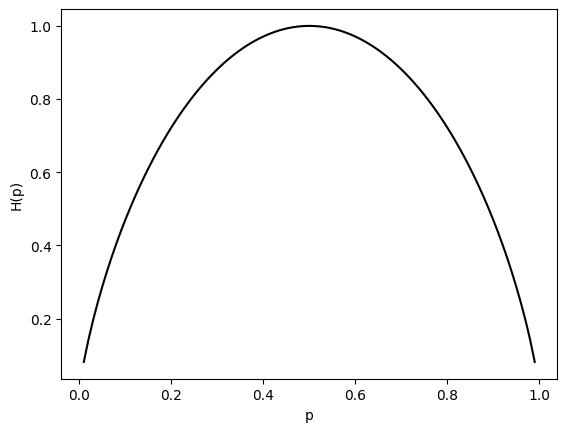
\includegraphics[width = 5.0cm]{entropy.png}
	\caption{$H(p) \mbox{vs.} p.$}
	\label{fig:entropy}
\end{figure}

\textgt{例 1.10}

\begin{align}
	X = \begin{cases}
		 & a\:\:\:\mbox{確率}\frac{1}{2}\mbox{のとき}, \\
		 & b\:\:\:\mbox{確率}\frac{1}{4}\mbox{のとき}, \\
		 & c\:\:\:\mbox{確率}\frac{1}{8}\mbox{のとき}, \\
		 & d\:\:\:\mbox{確率}\frac{1}{8}\mbox{のとき}.
	\end{cases}
\end{align}
エントロピーは
\begin{align}
	H(X) = - \left( \frac{1}{2} \log \frac{1}{2} + \frac{1}{4} \log \frac{1}{4} + \frac{1}{8} \log \frac{1}{8} + \frac{1}{8} \log \frac{1}{8} \right) = \frac{7}{4} \: \mbox{bits}
\end{align}

\section{Joint entropy and conditional entropy}

1章では, 単一の確率変数のエントロピーを定義した. ここでは, 確率変数のペアに対して定義を拡張する. この定義には特に新しいことはないが, $(X, Y)$は単一のベクトル値確率変数と見なすことができる.\\

\begin{itembox}[l]{\textgt{定義 2.1} (同時エントロピー)}
	同時エントロピー(joint entropy) $H(X, Y)$は, 同時分布(joint distribution) $p(x, y)$を持つ2つの確率変数$(X, Y)$について次のように定義される.
	\begin{align}
		H(X, Y) = - \sum_{x \in \mathcal{X}} \sum_{y \in \mathcal{Y}} p(x, y) \log p(x, y)
	\end{align}
\end{itembox}\\

また次式のようにも表される.
\begin{align}
	H(X, Y) = - E \log p(X, Y)
\end{align}\\

また, ある確率変数に別の確率変数が与えられたときの条件付きエントロピーを, 条件付き確率変数で平均した条件付き分布のエントロピーの期待値として定義する.\\

\begin{itembox}[l]{\textgt{定義 2.2} (条件付きエントロピー)}
	条件付きエントロピー(conditional entropy) $H(X|Y)$は次のように定義される.
	\begin{align}
		H(Y | X) & = \sum_{x \in \mathcal{X}} p(x) H(Y | X = x)                                      \\
		         & = - \sum_{x \in \mathcal{X}} p(x) \sum_{y \in \mathcal{Y}} p(y | x) \log p(y | x) \\
		         & = - \sum_{x \in \mathcal{X}} \sum_{y \in \mathcal{Y}} p(x, y) \log p(y | x)       \\
		         & = -E \log p(Y|X).
	\end{align}
\end{itembox}\\

同時エントロピーと条件付きエントロピーの定義の自然さは, 次の定理によって示される.\\

\begin{itembox}[l]{\textgt{定理 2.3} (エントロピーのチェイン則)}
	\begin{equation}
		H(X, Y) = H(X) + H(Y | X)
	\end{equation}
\end{itembox}\\

\textgt{証明 2.4} 定理 2.3の証明

\begin{align}
	H(X, Y) & = - \sum_{x \in \mathcal{X}} \sum_{y \in \mathcal{Y}} p(x, y) \log p(x, y)                                                                        \\
	        & = - \sum_{x \in \mathcal{X}} \sum_{y \in \mathcal{Y}} p(x, y) \log p(x) p(y | x)                                                                  \\
	        & = - \sum_{x \in \mathcal{X}} \sum_{y \in \mathcal{Y}} p(x, y) \log p(x) - \sum_{x \in \mathcal{X}} \sum_{y \in \mathcal{Y}} p(x, y) \log p(y | x) \\
	        & = - \sum_{x \in \mathcal{X}} p(x) \log p(x)- \sum_{x \in \mathcal{X}} \sum_{y \in \mathcal{Y}} p(x, y) \log p(y | x)                              \\
	        & = H(X) + H(Y|X).
\end{align}\qed\\

同等に次のように書くことができる.

\begin{align}
	\log p(X, Y) =\log p(X) + \log p(Y | X)
\end{align}\\

\begin{itembox}[l]{\textgt{系 2.5}}
	\begin{equation}
		H(X, Y|Z) = H(X|Z) + H(Y|X, Z)
	\end{equation}
\end{itembox}\\

\textgt{証明 2.6} 系 2.5の証明

\begin{align}
	H(X, Y|Z) & = - \sum_{z \in \mathcal{Z}} p(z) \sum_{x \in \mathcal{X}} \sum_{y \in \mathcal{Y}} p(x, y|z) \log p(x, y|z)               \\
	          & = - \sum_{z \in \mathcal{Z}} p(z) \sum_{x \in \mathcal{X}} \sum_{y \in \mathcal{Y}} p(x|z) p(y|x, z) \log p(x|z) p(y|x, z) \\
	\begin{split}
		& = - \sum_{z \in \mathcal{Z}} p(z) \sum_{x \in \mathcal{X}} \sum_{y \in \mathcal{Y}} p(x|z) p(y|x, z) \log p(x|z)\\
		& \quad \quad - \sum_{z \in \mathcal{Z}} p(z) \sum_{x \in \mathcal{X}} \sum_{y \in \mathcal{Y}} p(x|z) p(y|x, z) \log p(y|x, z)
	\end{split}                                                                                                             \\
	\begin{split}
		& = - \sum_{z \in \mathcal{Z}} p(z) \sum_{x \in \mathcal{X}} p(x|z) \log p(x|z)\\
		& \quad \quad - \sum_{z \in \mathcal{Z}} p(z) p(x|z) \sum_{x \in \mathcal{X}} \sum_{y \in \mathcal{Y}}  p(y|x, z) \log p(y|x, z)
	\end{split}                                                                                                             \\
	          & = H(X|Z) + H(Y|X,Z).
\end{align}\qed\\

\textgt{例 2.7} (X, Y)を次の同次分布とする.

\begin{table}[H]
	\centering
	\label{tab:hogehoge}
	\begin{tabular*}{10cm}{@{\extracolsep{\fill}}c|cccc}
		\diagbox{$Y$}{$X$} & 1             & 2 & 3 & 4 \\
		\hline
		1                  & $\frac{1}{8}$          & $\frac{1}{16}$ & $\frac{1}{32}$ & $\frac{1}{32}$ \\
		2                  & $\frac{1}{16}$         & $\frac{1}{8}$ & $\frac{1}{32}$ & $\frac{1}{32}$ \\
		3                  & $\frac{1}{16}$             & $\frac{1}{16}$ & $\frac{1}{16}$ & $\frac{1}{16}$ \\
		4                  & $\frac{1}{4}$             & 0 & 0 & 0 \\
	\end{tabular*}
\end{table}

$X$, $Y$の周辺分布はそれぞれ$(\frac{1}{2},\frac{1}{4},\frac{1}{8},\frac{1}{8})$,$(\frac{1}{4},\frac{1}{4},\frac{1}{4},\frac{1}{4})$であり, よって$H(X) = \frac{7}{4}$ bits, $H(Y) = 2$ bitsとなる. また,

\begin{align}
	H(X|Y) & = \sum_{i = 1}^{4} p(Y = i) H(X|Y=i)                                                                                                                                                                                                   \\
	       & = \frac{1}{4} H(\frac{1}{2}, \frac{1}{4}, \frac{1}{8}, \frac{1}{8}) + \frac{1}{4} H(\frac{1}{4}, \frac{1}{2}, \frac{1}{8}, \frac{1}{8}) + \frac{1}{4} H(\frac{1}{4}, \frac{1}{4}, \frac{1}{4}, \frac{1}{4}) + \frac{1}{4}H(0, 0, 0, 0) \\
	       & = \frac{1}{4} \times \frac{7}{4} + \frac{1}{4} \times \frac{7}{4} +  \frac{1}{4} \times 2 + \frac{1}{4} \times 0                                                                                                                       \\
	       & = \frac{11}{8} \mbox{bits}.
\end{align}

さらに, 定理 2.3 より

\begin{align}
	H(X, Y) & = H(X|Y) + H(Y)            \\
	        & = \frac{11}{8} + 2         \\
	        & = \frac{27}{8} \mbox{bits}
\end{align}\\

を得られる.\\

\textgt{解説 2.8} $H(Y|X) \neq H(X|Y)$ であるが, $H(Y) - H(Y|X) = H(X) - H(X|Y)$

\begin{align}
	\mbox{(左辺)} & = H(Y) - H(Y|X)                                       \\
	              & \stackrel{\mathrm{定理 2.3}}{=} H(Y) + H(Y) - H(X, Y) \\
	              & \stackrel{\mathrm{定理 2.3}}{=} H(X) -H(Y|X)          \\
	              & = \mbox{(右辺)}
\end{align}\qed

%%参考文献%%
%\newpage
\begin{thebibliography}{99}
	\bibitem{text}T.M.Cover and J.A.Thomas, Elements of Information Theory, Second Edition, John Wiley \& Sons, 2006.
\end{thebibliography}

\end{document}
